\documentclass[12pt,a4paper]{article}

% set font encoding for PDFLaTeX or XeLaTeX
\usepackage{ifxetex}
\ifxetex
  \usepackage{fontspec}
\else
  \usepackage[T1]{fontenc}
  \usepackage[utf8]{inputenc}
  \usepackage{lmodern}
\fi

\usepackage[utf8]{inputenc} % per a poder fer servir accents
\usepackage[catalan]{babel} % idioma per les coses automà tiques
\usepackage{amssymb}        % símbols de l'AMS
\usepackage{amsmath}        % macros de l'AMS
\usepackage{amsbsy}
\usepackage{amsthm}
\usepackage{dsfont}
\usepackage[all]{xy}           % diagrames
\usepackage[pdftex]{graphicx}  % poder incloure gràfics
\usepackage[pdftex]{color}     % poder fer servir color al text

\usepackage{hyperref} %referencies

\newtheorem{prop}{Proposició}
\newtheorem{teor}{Teorema}


% used in maketitle
\title{El meu treball de \LaTeX}
\author{Mireia Gómez i Diaz}
\date{}

% Enable SageTeX to run SageMath code right inside this LaTeX file.
% documentation: http://mirrors.ctan.org/macros/latex/contrib/sagetex/sagetexpackage.pdf
% \usepackage{sagetex}

\begin{document}
\maketitle
\tableofcontents
\section{Introducció}
L’objectiu d’aquest treball és avaluar el coneixement de l’editor de text \LaTeX. A la Secció \ref{s:s2} hi utilitzem un tema d’Àlgebra Lineal i a la Secció \ref{s:s3} un de Càlcul Diferencial.

\section{Àlgebra Lineal} \label{s:s2}
En aquesta secció recordem algunes propietats de la matriu associada a una aplicació lineal. En cap moment pretenem ser exhaustius. Per a aprofundir en el tema referim el lector a l’assignatura \textit{Àlgebra lineal} del primer curs de Grau de Matemàtiques i a la bibliografia d’aquesta assignatura com ara per exemple \cite{cedo}, \cite{merino}. La pàgina web interactiva \cite{gomez} és un recurs més bàsic on s’expliquen pas a pas les nocions d’Àlgebra Lineal amb molts exemples i il·lustracions.

\subsection{Aplicacions Lineals}
En tota la secció suposem que
\begin{itemize}
\item \textit{V,W} són espais vectorials sobre $\mathbb{R}$.
\item $\mathcal{B}=\left\lbrace v_{1},\ldots, v_{n} \right\rbrace$ és una base ordenada de \textit{V}.
\item $\overline{\mathcal{B}}=\left\lbrace w_{1},\ldots, w_{m} \right\rbrace$ és una base ordenada de \textit{W}.
\item $T: V \rightarrow W$ és una aplicació lineal entre els espais vectorials \textit{V} i \textit{W}.
\end{itemize}

\paragraph{\textbf{Coordenades d'un vector.}} Per cada vector $v \in V$ existeixen $x_{1},\ldots, x_{n} \in \mathbb{R}$ únics de manera que $v=\sum_{i=1}^{n}x_{i}v_{i}$. El vector $(x_{1},\ldots,x_{n})$ s'anomena vector de les coordenades de $v$ respecte de la base $\mathcal{B}$, i el denotem per

\begin{equation}
\left[v\right]_{\mathcal{B}}=(x_{1},\ldots,x_{n}).
\end{equation}

\paragraph{\textbf{Matriu associada a una aplicació lineal.}} La matriu associada a $T$ respecte de les bases $\mathcal{B}$ en $\overline{\mathcal{B}}$ està donada per
\begin{equation}
m(T)_{\mathcal{B},\overline{\mathcal{B}}}=\left( \
\begin{tabular}{|c|c|c|c|}
\hline & & &\\
 $\left[T(v_{1})\right]_{\overline{\mathcal{B}}}$ & $\left[T(v_{2})\right]_{\overline{\mathcal{B}}}$ & $\ldots$ & $ \left[T(v_{n})\right]_{\overline{\mathcal{B}}}$ \\
  & & &  \\
\hline
\end{tabular}
\ \right)
\end{equation}
on la $i$-èsima columna està formada per les coordenades de $T(v_{i})$ respecte de la base $\overline{\mathcal{B}}$. Notem que, per cada $v \in V$, les coordenades de $T(v)$ respecte de $\overline{\mathcal{B}}$ estan donades per
\begin{equation} \label{eq:eq3}
\left[T(v)\right]_{\overline{\mathcal{B}}} = m(T)_{\mathcal{B},\overline{\mathcal{B}}} \cdot \left[v\right]_{\mathcal{B}},
\end{equation}
on els vectors de coordenades $\left[v\right]_{\mathcal{B}}$ i $\left[T(v)\right]_{\overline{\mathcal{B}}}$ estan considerats com matrius de dimensió $n \times 1$ i $m \times 1$ respectivament. Aleshores, si $\left[T(v)\right]_{\overline{\mathcal{B}}} = (y_{1},\ldots,y_{m})$, llavors $T(v)=\sum_{i=1}^{m}y_{i}w_{i}$.

\paragraph{\textbf{Matriu de l'aplicació lineal inversa.}} Si $T: V \rightarrow W$ és un isomorfisme, aleshores dim$V$=dim$W$, $m(T)_{\mathcal{B},\overline{\mathcal{B}}}$ és invertible i la seva matriu inversa és:
$$ \left(m(T)_{\mathcal{B},\overline{\mathcal{B}}}\right)^{-1} = m(T^{-1})_{\mathcal{B},\overline{\mathcal{B}}}.$$
Esquemàticament,
\begin{equation}
\xymatrix{ \left[v\right]_{\mathcal{B}} \ar@/^2pc/[rr]^{m(T)_{\mathcal{B},\overline{\mathcal{B}}}} & & \left[T(v)\right]_{\overline{\mathcal{B}}} \ar@/^2pc/[ll]^{m(T^{-1})_{\mathcal{B},\overline{\mathcal{B}}}}}
\end{equation}
on tenim a l'esquerra les coordenades del vector $v$ respecte de la base $\mathcal{B}$ i a la dreta les coordenades del vector $T(v)$ respecte de la base $\overline{\mathcal{B}}$.

\paragraph{\textbf{Teorema fonamental de les transformacions lineals}} El teorema següent dóna condicions suficients i necessàries perquè existeixi una aplicació lineal única que transforma una figura geomètrica donada en una altra. Després, com a il·lustració, treballarem un exemple en l'espai vectorial $\mathbb{R}^{2}$.

\begin{teor} \label{teo:teo1}
Siguin $V,W$ espais vectorials, sigui $\mathcal{B}= \left\lbrace v_{1}, v_{2},\ldots, v_{n}\right\rbrace$ una base de V i siguin $w_{1}, w_{2},\ldots,w_{n}$ vectors arbitraris (iguals o no) de $W$. Aleshores existeix una única aplicació lineal $T: V \rightarrow W$ que compleix $T(v_{i})=w_{i}$, $1 \leq i \leq n$.
\end{teor}

La demostració d'aquest teorema es pot trobar a \cite{cedo}. Tot seguit expliquem com trobar l'aplicació $T$ en un cas concret.

Anem a veure si podem transformar el triangle que hi ha a l’esquerra en el triangle que hi ha a la dreta de l’esquema (\ref{eq:eq5}):
\begin{equation} \label{eq:eq5}
\xymatrix{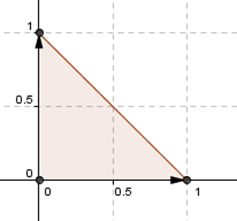
\includegraphics[width=3cm]{Teoremafund1.png} \ar@/_2pc/[rr]^{T} & & 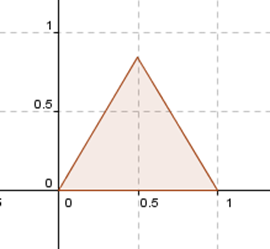
\includegraphics[width=3cm]{Teoremafund2.png}}
\end{equation}
Pel Teorema \ref{teo:teo1}, una aplicació lineal és determinada únicament per les imatges d'una base de $\mathbb{R}^{2}$. Observem que la base canònica, $\mathcal{B}= \left\lbrace (1,0),(0,1) \right\rbrace$, determina el primer triangle. D'acord amb això, li assignem les següents imatges transformades per $T$:
$$ \left\{ \begin{array}{lcc}
             T((1,0))  & = (1,0), \\
             \\ T((0,1)) &  = (\frac{1}{2},1).
             \end{array}
   \right.  $$
Per trobar la forma analítica de l'aplicació lineal $T$ podem utilitzar (\ref{eq:eq3}) tot observant que les coordenades són els vectors mateixos si triem com a bases ordenades $\mathcal{B}=\overline{\mathcal{B}}$ la base canònica de $V = W = \mathbb{R}^{2}$. Sigui $v=(x,y)$ un vector genèric de $\mathbb{R}^{2}$, aleshores la seva imatge transformada per $T$ és:
$$ T((x,y))= m(T)_{\mathcal{B},\overline{\mathcal{B}}} \cdot {\begin{pmatrix}
x\\
y
\end{pmatrix}} =
{\begin{pmatrix}
x+\frac{1}{2}y\\
y
\end{pmatrix}} = (x+\frac{1}{2}y,y).$$

\section{Càlcul diferencial} \label{s:s3}
Recordem aquí una propietat de la derivada de funcions d'una variable.
\begin{prop}
Suposem que r $>1$ és una constant i $f: I \subset \mathbb{R} \rightarrow \mathbb{R}$ és una funció que compleix la desigualtat $f(x) \leq |x|^{r}$ per cada x en I, on I és un interval obert que conté $0$. Aleshores f és diferenciable en $x=0$.
\end{prop}


\begin{proof}
La desigualtat $f(x)\leq|x|^{r}$ amb $r>1$ implica que $f(0)=0$. Per tant tenim que
$$\left|\dfrac{f(x)-f(0)}{x-0}\right|=\left|\dfrac{f(x)}{x}\right|\leq|x|^{r-1}.$$
Com que $r-1>0$, tenim que $\lim\limits_{x \to 0}|x|^{r-1}=0$, per la qual cosa obtenim que
\begin{equation} \label{eq:eq6}\begin{split}
\lim_{x \to 0}\left|\dfrac{f(x)-f(0)}{x-0}\right| \\\ \Leftrightarrow \lim_{x \to 0}\dfrac{f(x)-f(0)}{x-0}.
\end{split} \end{equation}
Llavors, d'acord amb la definició de diferenciabilitat, (\ref{eq:eq6}) diu que $f$ és diferenciable en $x=0$ amb $f'(0)=0$.
\end{proof}





\begin{thebibliography}{99\kern2pt}
%\bibliographystyle{plain}
\setlength\itemsep{-1pt}

\newcommand\vvv{\unskip, }
\newcommand\nnn{\unskip, n.\,}
\newcommand\ppp{\unskip\,: }

\bibitem{cedo}
F. Cedo, A. Reventós.
\textit{Geometria plana i Àlgebra lineal}. Manuals de la UAB, Servei de Publicacions, UAB, Bellaterra, 2004.

\bibitem{merino}
L. Merino i E. Santos.
\textit{Álgebra lineal con métodos elementales}. Ed. Thomson, Madrid, 2006.

\bibitem{gomez}
F. Gómez, I. Pustilnik.
\textit{Álgebra y Geometría Analítica Online!}
\url{https://aga.frba.utn.edu.ar}, 2017.



\end{thebibliography}




\end{document}
